\subsection{Heuristics Analysis}
    We first look at the effect of considering only Operations after a specific start timestamp for computing \texttt{Pad} heuristics and compare it  to the score that considers \texttt{Operations} from the start. Then we see how \texttt{Paragraph} number and \texttt{Superparagraph} length evolve in time and we use time series analysis to see whether we could use these metrics to predict how much longer the students will take to finish the task.
    \subsubsection{Comparison between full Pad and window scores}
        We presented the need for modifying the scores that we were computing in the previous version of the tool so that the changes introduced by new \texttt{Operations} have a more noticeable impact.
        However, we need to keep in mind that some \texttt{Operations} may not be considered when using the window-contained Operations approach, particularly if some \texttt{Operations} are not fully contained within a single time window.

        Figures \ref{fig:typeoverallscorewrite} and \ref{fig:windowtypeoverallscorewrite} show the overall scores for writing operations, both using the defined time interval of 3 minutes. These Figures show in gray the boxplots of the score values per window for all pads, and in blue the average value with the standard deviation error bars.
    
        \begin{figure}[htp!]
            \centering
            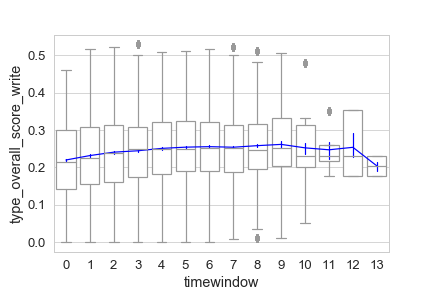
\includegraphics[width=0.5\textwidth]{figures/typeoverallscorewrite.png}
            \caption{Overall score for write type using 3 min time windows and considering Operations from the beginning of the Pad.}
            \label{fig:typeoverallscorewrite}
        \end{figure}
        \begin{figure}[htp!]
            \centering
            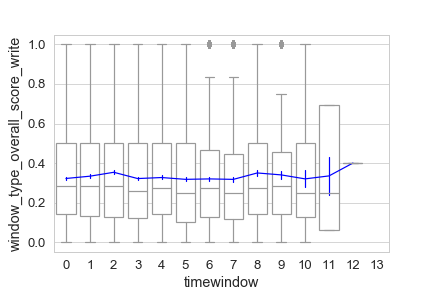
\includegraphics[width=0.5\textwidth]{figures/windowtypeoverallscorewrite.png}
            \caption{Overall score for write type using 3 min time windows and considering Operations from the beginning of the window (new implementation).}
            \label{fig:windowtypeoverallscorewrite}
        \end{figure}
        
        In Figure \ref{fig:typeoverallscorewrite} the line is smoother, as we are considering all the Operations from the beginning of the Pad until the end of the current window and therefore at every window we are averaging any possible changes with the rest of the Pad. Figure \ref{fig:windowtypeoverallscorewrite} shows the score changes from one window to another more clearly, as it is only considering the Operations within the time window. 
        
    \subsubsection{Paragraph and Superparagraph length in time} 
    In this section we decided to look at the number of paragraphs per superparagraph and at the average paragraph length and how these metrics change in time. We decided to try a simple model to see how well it could fit our data, and the results are shown in Figures \ref{fig:avg_p_sp} and \ref{fig:avg_len_p}. In both cases we decided to fit the values observed that correspond to windows 0 to 13, as windows 14 to 17 have less observations (because most paragraphs last 45 minutes or less, i.e. they last only 15 timewindows). However, we plot the results for windows 15 to 17 as well.
    
        \begin{figure}[htp!]
            \centering
            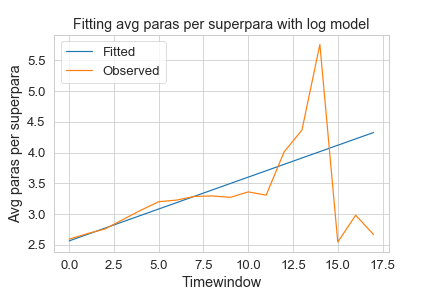
\includegraphics[width=0.5\textwidth]{figures/avg_p_sp.png}
            \caption{Average number of Paragraphs per Superparagraph. The linear model fitted has slope 0.1 and offset 2.55.}
            \label{fig:avg_p_sp}
        \end{figure}
        \begin{figure}[htp!]
            \centering
            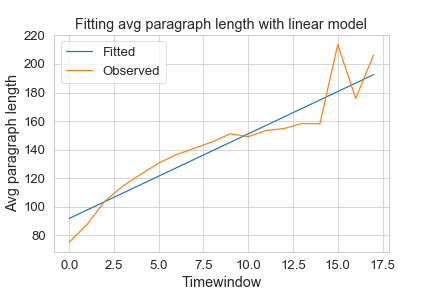
\includegraphics[width=0.5\textwidth]{figures/avg_len_p.png}
            \caption{Average length in characters per Paragraph. The linear model fitted has slope 5.9 and offset 91.8.}
            \label{fig:avg_len_p}
        \end{figure}
    
    From the two metrics obtained here we could obtain the value of the average Superparagraph length, as it would be the product of both.
    
    We see that the tendency does not seem to converge, so from these results we would not be able to say whether we could predict when the task will be finished. However, we need to keep in mind that the average for first windows has been computed over more pads than for the last windows. As we can see, up until timewindow 11 (which would correspond to minute 33 of the task), it seems like the values would converge. For this reason, it may be interesting to repeat this analysis after implementing a different WindowOperation split that takes into account the total duration of the pad.